\documentclass[hidelinks]{article}

\usepackage{van-de-la-sehen-en}
\usepackage{van-de-environnement-en}
\usepackage{boite/van-de-boite-en}
\usepackage{van-de-abbreviation}
\usepackage{van-de-neko}
\usepackage{van-le-trompe-loeil}
\usepackage{cyanide/van-de-cyanide}
\usepackage[most]{tcolorbox}
\usepackage{van-le-trompe-loeil}
\usepackage{cmbright}
\usepackage{nccmath}
\usepackage[paperheight=297mm,paperwidth=240mm,top=.2in,left=.1in,right=.1in,bottom=.2in, landscape]{geometry}
\usepackage{tensor}

\definecolor{graybg}{RGB}{242,241,236}
\definecolor{titlepurple}{RGB}{138,47,57}
\definecolor{shadegray}{RGB}{102,119,136}
\definecolor{itemgray}{RGB}{163,149,128}
\definecolor{mathnormalblack}{RGB}{0,0,0}
\definecolor{textblack}{RGB}{72,72,72}
\pagecolor{graybg}

\usepackage{multicol}
\setlength{\columnsep}{.1in}

\newcommand{\raisedrule}[2][0em]{\qquad}
%\leaders\hbox{\rule[#1]{1pt}{#2}}\hfill}
\newcommand{\wdiv}{\,·\,}

\setlength{\parindent}{0pt}

\newcommand{\titlefont}{\tt }
\newcommand{\mathtextfont}{\mysans }
\newcommand{\emphbox}[1]{\colorbox{lightgray!20}{$\displaystyle #1$}}

\newdimen\indexlen
\def\newheader#1{%
\def\probindex{#1}
\setlength\indexlen{\widthof{\Large\color{titlepurple}\mysans #1\qquad}}
\vspace{1em}
\mbox{{\Large\color{titlepurple}\mysans #1\qquad}
\raisebox{.5em}{\tikz \fill[titlepurple,opacity=.2,path fading=east] (0,0.05em) rectangle (\dimexpr\linewidth-\indexlen\relax,0em);}}
}
\def\newsimpheader#1{%
\vspace{1em}
{\Large\color{titlepurple} #1\qquad}\newline
}
\def\mathitem#1{\text{\color{itemgray}\mysans #1}}
\def\mathcomment#1{\text{\color{lightgray}\quad \texttt{\#}\kern-0pt#1}}
\def\mathheadcomment#1{\text{\color{lightgray}\texttt{\#}\kern-0pt#1}}
\def\midbreak{\smash{\raisebox{1.5em}{\smash{\tikz \path[opacity=.2,left color=white,right color=white,middle color=black] (0,0.05em) rectangle (\linewidth,0em);}}}
\vspace{-4em}}
\newtcolorbox{cheatresume}{enhanced, arc=.5pt, left=.5em, frame hidden, boxrule=0pt, colback=white, fuzzy halo=.05pt with lightgray, shadow={.4pt}{-.4pt}{0pt}{fill=shadegray,opacity=0.3}}

\usepackage{stackengine}
\stackMath
\usepackage{scalerel}
\usepackage[outline]{contour}

\newlength\thisletterwidth
\newlength\gletterwidth
\newcommand{\leftrightharpoonup}[1]{%
{\ooalign{$\scriptstyle\leftharpoonup$\cr%\kern\dimexpr\thisletterwidth-\gletterwidth\relax
$\scriptstyle\rightharpoonup$\cr}}\relax%
}
\def\tensor#1{\settowidth\thisletterwidth{$\mathbf{#1}$}\settowidth\gletterwidth{$\mathbf{g}$}\stackon[-0.1ex]{\mathbf{#1}}{\boldsymbol{\leftrightharpoonup{#1}}}  }
\def\mitensor#1{\stackon[-0.1ex]{\+v#1}{\boldsymbol{\leftrightharpoonup{#1}}} }
\def\onedot{$\mathsurround0pt\ldotp$}
\def\cddot{% two dots stacked vertically
:}%

\newcommand*{\mysans}{\fontfamily{phv}\selectfont}
\definecolor{emphgreen}{RGB}{238,255,207}
%\newcommand{\resume}[1]{\par
%\noindent\colorbox{emphgreen}{#1}}

    \tikzset{
    partial ellipse/.style args={#1:#2:#3}{
        insert path={+ (#1:#3) arc (#1:#2:#3)}
    }}

\usepackage{physics}
\usepackage{bbm}

\definecolor{elementorange}{RGB}{251,123,21}
\definecolor{elementlightblue}{RGB}{129,178,214}
\definecolor{elementred}{RGB}{254,3,0}
\definecolor{elementO}{RGB}{254,3,0}

\definecolor{elementblue}{RGB}{34,71,220}
\definecolor{elementbrown}{RGB}{181,113,0}

\definecolor{elementTi}{RGB}{120,202,255}
\definecolor{elementCa}{RGB}{90,221,189}

\definecolor{elementCu}{RGB}{34,71,220}

\definecolor{elementCa2}{RGB}{90,150,189}
\definecolor{elementF}{RGB}{176,185,230}

\definecolor{elementFe}{RGB}{181,113,0}
\definecolor{elementS}{RGB}{255,250,0}

\definecolor{elementNa}{RGB}{249,220,60}
\definecolor{elementCl}{RGB}{49,252,2}

\definecolor{elementCs}{RGB}{14,254,185}

\definecolor{elementZn}{RGB}{143,143,129}
\definecolor{elementW}{RGB}{141,138,127}
\definecolor{elementSi}{RGB}{27,59,250}
\definecolor{elementMg}{RGB}{251,123,21}

\begin{document}

\begin{multicols*}{3}[\centerline{\titlefont Crystal Structures}]
\raggedcolumns%
\newheader{Tenary}
\begin{cheatresume}
\begin{tabular}{cc}
    \mathitem{Spinel} & \mathitem{Inverse Spinel} \\
    \includegraphics[width=.4\textwidth]{src/Spinel.png} & \includegraphics[width=.4\textwidth]{src/Cuprospinel.png} \\
    \color{textblack}\ce{MgAl2O4} & \color{textblack}\ce{CuFe2O4} \\
    \color{textblack}\tikz\draw[draw=none,red,fill=elementorange] (0,0) circle (.3em);\,\tikz\draw[draw=none,red,fill=elementlightblue] (0,0) circle (.3em);\textsubscript{2}\tikz\draw[draw=none,red,fill=elementred] (0,0) circle (.3em);\textsubscript{4} & \color{textblack}\tikz\draw[draw=none,red,fill=elementblue] (0,0) circle (.3em);\,\tikz\draw[draw=none,red,fill=elementbrown] (0,0) circle (.3em);\textsubscript{2}\tikz\draw[draw=none,red,fill=elementred] (0,0) circle (.3em);\textsubscript{4} \\[.5em]
    \mathitem{Perovskite} \\
    \includegraphics[width=.4\textwidth]{src/Perovskite.png} \\
    \color{textblack}\ce{CaTiO3} \\
    \color{textblack}\tikz\draw[draw=none,red,fill=elementCa] (0,0) circle (.3em);\,\tikz\draw[draw=none,red,fill=elementTi] (0,0) circle (.3em);\,\tikz\draw[draw=none,red,fill=elementO] (0,0) circle (.3em);\textsubscript{3}
\end{tabular}
\end{cheatresume}
\newheader{AB\textsubscript{2}}
\begin{cheatresume}
\begin{tabular}{cc}
    \mathitem{Rutile} & \mathitem{Cuprite} \\
    \includegraphics[width=.4\textwidth]{src/Rutile.png} & \includegraphics[width=.4\textwidth]{src/Cuprite.png} \\
    \color{textblack}\ce{TiO2} & \color{textblack}\ce{Cu2O} \\
    \color{textblack}\tikz\draw[draw=none,red,fill=elementTi] (0,0) circle (.3em);\,\tikz\draw[draw=none,red,fill=elementO] (0,0) circle (.3em);\textsubscript{2} & \color{textblack}\tikz\draw[draw=none,red,fill=elementCu] (0,0) circle (.3em);\textsubscript{2}\tikz\draw[draw=none,red,fill=elementO] (0,0) circle (.3em); \\[.5em]
    \mathitem{Fluorite} & \mathitem{Pyrite} \\
    \includegraphics[width=.4\textwidth]{src/Fluorite.png} & \includegraphics[width=.4\textwidth]{src/Pyrite.png} \\
    \color{textblack}\ce{CaF2} & \color{textblack}\ce{FeS2} \\
    \color{textblack}\tikz\draw[draw=none,red,fill=elementCa2] (0,0) circle (.3em);\,\tikz\draw[draw=none,red,fill=elementF] (0,0) circle (.3em);\textsubscript{2} & \color{textblack}\tikz\draw[draw=none,red,fill=elementFe] (0,0) circle (.3em);\,\tikz\draw[draw=none,red,fill=elementS] (0,0) circle (.3em);\textsubscript{2}
\end{tabular}
\end{cheatresume}
\columnbreak
\newheader{AB}
\begin{cheatresume}
\begin{tabular}{cc}
    \mathitem{NaCl} & \mathitem{CsCl} \\
    \includegraphics[width=.4\textwidth]{src/NaCl.png} & 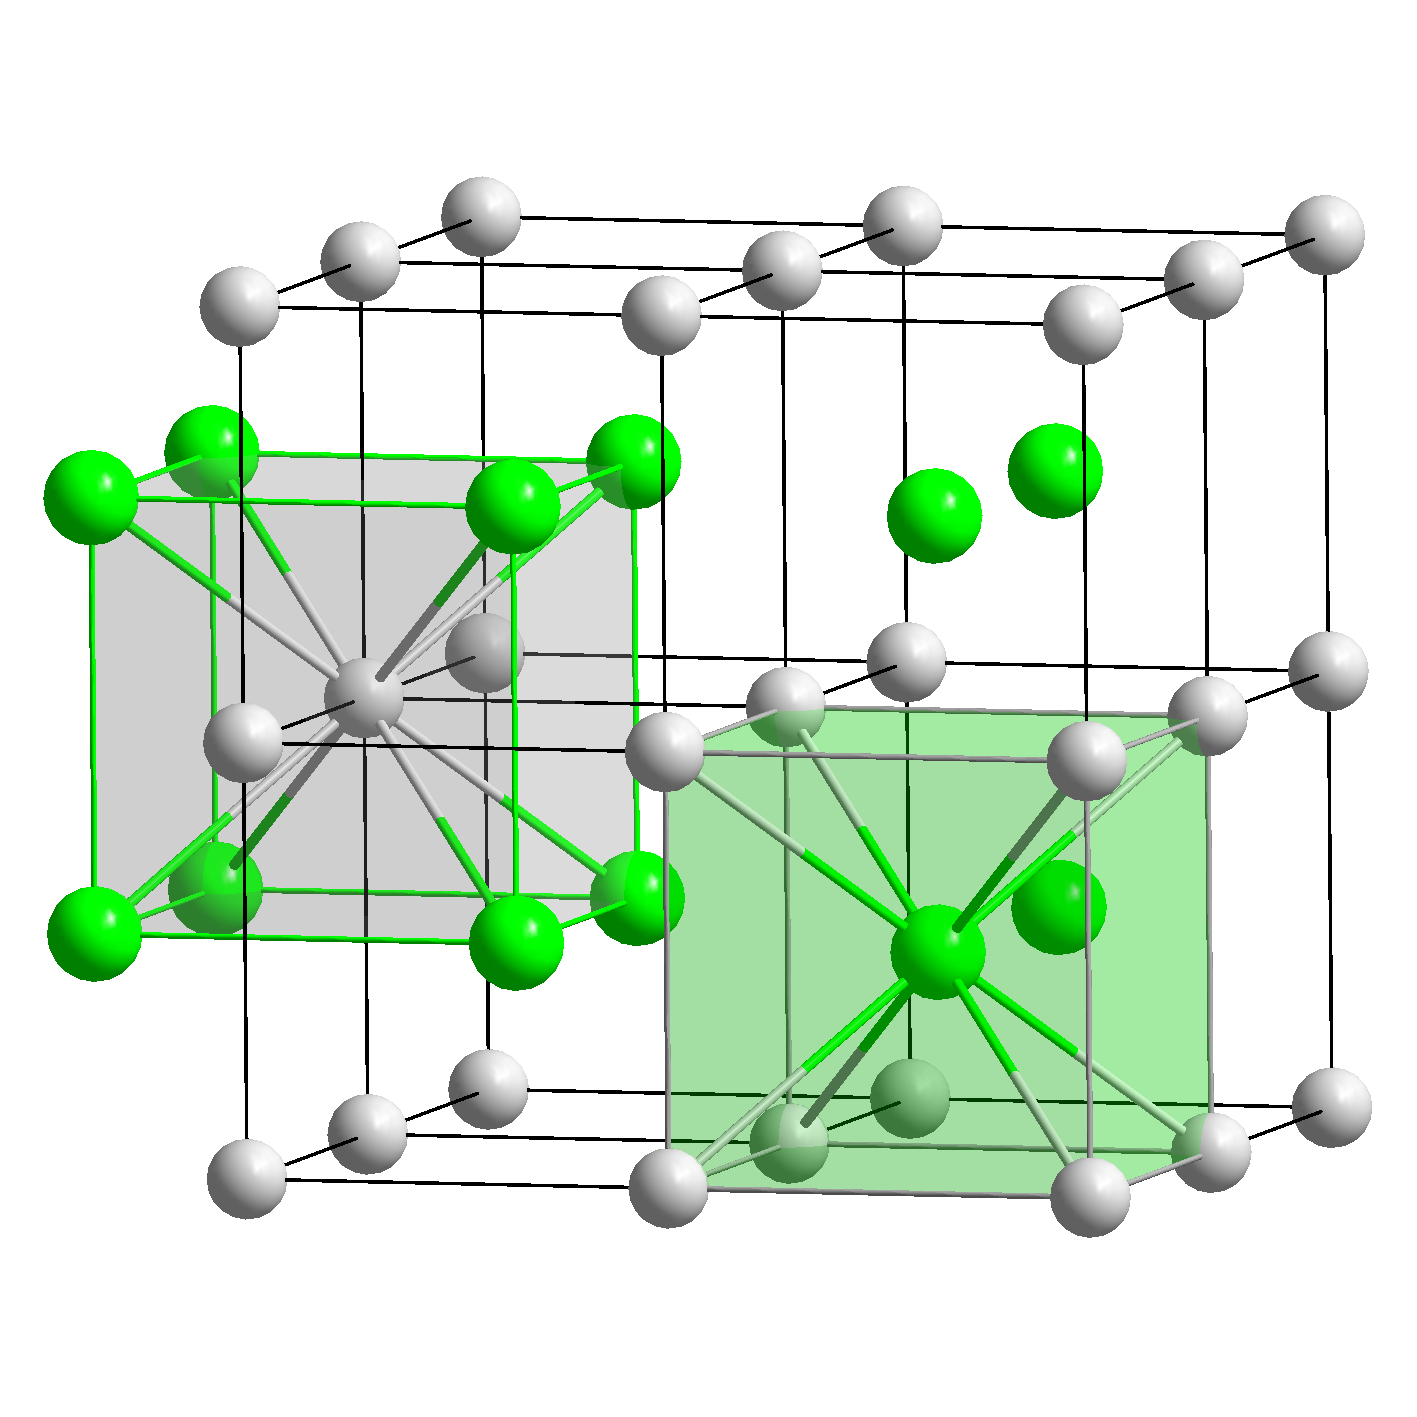
\includegraphics[width=.4\textwidth]{src/CsCl.png} \\
    \color{textblack}\ce{NaCl} & \color{textblack}\ce{CsCl} \\
    \color{textblack}\tikz\draw[draw=none,red,fill=elementNa] (0,0) circle (.3em);\,\tikz\draw[draw=none,red,fill=elementCl] (0,0) circle (.3em); & \color{textblack}\tikz\draw[draw=none,red,fill=elementCs] (0,0) circle (.3em);\,\tikz\draw[draw=none,red,fill=elementCl] (0,0) circle (.3em); \\[.5em]
    \mathitem{Sphalerite} & \mathitem{Wurtzite} \\
    \includegraphics[width=.4\textwidth]{src/Sphalerite.png} & \includegraphics[width=.4\textwidth]{src/Wurtzite.png} \\
    \color{textblack}\ce{ZnS} & \color{textblack}\ce{ZnS} \\
    \color{textblack}\tikz\draw[draw=none,red,fill=elementZn] (0,0) circle (.3em);\,\tikz\draw[draw=none,red,fill=elementS] (0,0) circle (.3em); & \color{textblack}\tikz\draw[draw=none,red,fill=elementZn] (0,0) circle (.3em);\,\tikz\draw[draw=none,red,fill=elementS] (0,0) circle (.3em);
\end{tabular}
\end{cheatresume}
\newheader{Element}
\begin{cheatresume}
\begin{tabular}{cc}
    \mathitem{FCC} & \mathitem{BCC} \\
    \includegraphics[width=.4\textwidth]{src/Cu.png} & \includegraphics[width=.4\textwidth]{src/W.png} \\
    \color{textblack}\ce{Cu} & \color{textblack}\ce{W} \\
    \color{textblack}\tikz\draw[draw=none,red,fill=elementCu] (0,0) circle (.3em); & \color{textblack}\tikz\draw[draw=none,red,fill=elementW] (0,0) circle (.3em); \\[.5em]
    \mathitem{Diamond} & \mathitem{HCP} \\
    \includegraphics[width=.4\textwidth]{src/Si.png} & \includegraphics[width=.4\textwidth]{src/Mg.png} \\
    \color{textblack}\ce{Si} & \color{textblack}\ce{Mg} \\
    \color{textblack}\tikz\draw[draw=none,red,fill=elementSi] (0,0) circle (.3em); & \color{textblack}\tikz\draw[draw=none,red,fill=elementMg] (0,0) circle (.3em);
\end{tabular}
\end{cheatresume}

\end{multicols*}

\end{document}
